\documentclass[a4paper, 12pt]{article}

\usepackage[left=2cm,right=2cm,
    top=2cm,bottom=2cm,bindingoffset=0cm]{geometry}

\usepackage[T2A]{fontenc}
\usepackage[utf8]{inputenc}
\usepackage{color}
\usepackage{graphicx}
\usepackage{caption}
\usepackage{subcaption}
\usepackage{tikz}
\usepackage[english, russian]{babel}
\usepackage{ gensymb }
\usepackage{booktabs}
\usepackage{amsmath,amsfonts,amssymb,amsthm,mathtools}
\usepackage{lscape}
\usepackage{listings}

\begin{document}


\begin{center}
\textbf{Метод конечных элементов для двумерной задачи теплопроводности.}
\end{center}
\begin{center}
\textbf{\textit{Задание}}
\end{center}

Решить задачу распространения тепла для области из 1 лабораторной работы. Тело разбить на треугольные симплекс элементы. Записать интегральную или вариационную формулировку задачи, показать алгоритм сведения к СЛАУ. Составить локальные матрицы жесткости и правых частей. Произвести сборку в глобальную матрицу и глобальный вектор. Решить СЛАУ.

\begin{center}
\textbf{\textit{Решение}}
\end{center}

\begin{enumerate}
\item Уравнение теплопроводности:
\[-\nabla(K\nabla T) = 0 \text{ в области } V\]

Граничное условие на $S$:
\[
K \frac{\partial T}{\partial n} + a_g (T - T_g) - q = 0
\]

Вариационная постановка:
\[
\int\limits_V -\nabla \cdot (K \nabla T) v dV = 0,
\]
где \( v \) — пробная функция. Применяя интегрирование по частям и теорему Гаусса-Остроградского, получаем функционал:
\begin{equation}\label{J}
J(T) = \int\limits_V \frac{1}{2} 
\left[ K_x \left( \frac{\partial T}{\partial x} \right)^2 + K_y \left( \frac{\partial T}{\partial y} \right)^2 \right] dV 
- \int\limits_{S_1} q T dS 
+ \int\limits_{S_2} \frac{1}{2} a_g (T - T_g)^2 dS
\end{equation}

Введем обозначения:
\begin{equation}\label{K}
K = 
\begin{pmatrix}
K_x & 0 \\
0 & K_y
\end{pmatrix}, 
\quad T = N_i T_i + N_j T_j + N_k T_k = N \Phi, \ \ 
\begin{pmatrix}
\displaystyle\frac{\partial T}{\partial x} \\ \\
\displaystyle\frac{\partial T}{\partial y}
\end{pmatrix} 
= 
\begin{pmatrix}
\displaystyle\frac{\partial N}{\partial x} \\ \\
\displaystyle\frac{\partial N}{\partial y}
\end{pmatrix} \Phi= B \Phi
\end{equation}

Тогда с учетом \eqref{K} перепишем \eqref{J}:
\[
J = \frac{1}{2} \int\limits_V \left[ \Phi^T B^T K B \Phi \right] dV - \int\limits_{S_1} q N \Phi dS + \frac{1}{2} \int\limits_{S_2} a_g (N \Phi - T_g)^2 dS
\]

Задача сводится к минимизации \( J(T) \to \min \):
\[
\frac{\partial J(T)}{\partial \Phi} = 0, \quad \Phi = (T_1, T_2, T_3)^T
\]

Следовательно:
\[
\int\limits_V B^T K B \Phi dV - \int\limits_{S_1} N^T q dS + \int\limits_{S_2} a_g N^T N \Phi dS - \int\limits_{S_2} a_g N^T T_g dS = 0
\]

Рведем обозначения:
\[
K = \int\limits_V B^T K B dV + \int\limits_{S_2} a_g N^T N dS, \quad F = \int\limits_{S_1} N^T q dS + \int\limits_{S_2} a_g N^T T_g dS
\]

Решение задачи сводится к решению СЛАУ \( K \Phi = F \).

Задача решается с использованием симлексного трехузлового конечного элемента.
\begin{equation}\label{T}
T = a_1 + a_2 x + a_3 y
\end{equation}
\[
\begin{cases}
T_i = \alpha_1 + \alpha_2 x_i + \alpha_3 y_i, \\
T_j = \alpha_1 + \alpha_2 x_j + \alpha_3 y_j, \\
T_k = \alpha_1 + \alpha_2 x_k + \alpha_3 y_k 
\end{cases}
\]

Решим систему методом Крамера:
\[
\Delta = 
\begin{vmatrix}
1 & x_i & y_i \\
1 & x_j & y_j \\
1 & x_k & y_k \\
\end{vmatrix}
= 2S, \quad S \text{ — площадь треугольника.}
\]

\[
\Delta_1 = 
\begin{vmatrix}
T_i & x_i & y_i \\
T_j & x_j & y_j \\
T_k & x_k & y_k \\
\end{vmatrix}
= T_i \underbrace{(x_j y_k - x_k y_j)}_{a_i} + T_j \underbrace{(x_k y_i - x_i y_k)}_{a_j} + T_k \underbrace{(x_i y_j - x_j y_i)}_{a_k}
\]

\[
\Delta_2 = 
\begin{vmatrix}
1 & T_i & y_i \\
1 & T_j & y_j \\
1 & T_k & y_k \\
\end{vmatrix}
= T_i \underbrace{(y_j - y_k)}_{b_i} + T_j \underbrace{(y_k - y_i)}_{b_j} + T_k \underbrace{(y_i - y_j)}_{b_k}
\]

\[
\Delta_3 = 
\begin{vmatrix}
1 & x_i & T_i \\
1 & x_j & T_j \\
1 & x_k & T_k \\
\end{vmatrix}
= T_i \underbrace{(x_k - x_j)}_{c_i} + T_j \underbrace{(x_i - x_k)}_{c_j} + T_k \underbrace{(x_j - x_i)}_{c_k}
\]

Тогда \(\displaystyle \alpha_1 = \frac{\Delta_1}{\Delta}, \, \alpha_2 = \frac{\Delta_2}{\Delta}, \, \alpha_3 = \frac{\Delta_3}{\Delta} \). Подставим в \eqref{T}:
\[
T = \frac{1}{\Delta} \left( T_i (a_i + b_i x + c_i y) + T_j (a_j + b_j x + c_j y) + T_k (a_k + b_k x + c_k y) \right) 
= N_i T_i + N_j T_j + N_k T_k = N \Phi,
\]

где
\[
\begin{cases}
\begin{aligned}
N_i &= \frac{1}{\Delta} (a_i + b_i x + c_i y), \\
N_j &= \frac{1}{\Delta} (a_j + b_j x + c_j y), \\
N_k &= \frac{1}{\Delta} (a_k + b_k x + c_k y)
\end{aligned}
\end{cases}
\]
— функции формы. Матрица \( B \):
\[
\begin{aligned}
\begin{pmatrix} \displaystyle
\frac{\partial N_i}{\partial x} &\displaystyle \frac{\partial N_j}{\partial x} &\displaystyle \frac{\partial N_k}{\partial x} \\ \\
\displaystyle\frac{\partial N_i}{\partial y} &\displaystyle \frac{\partial N_j}{\partial y} &\displaystyle \frac{\partial N_k}{\partial y} \\
\end{pmatrix} \Phi
= 
\frac{1}{\Delta} 
\begin{pmatrix} 
b_i & b_j & b_k \\
c_i & c_j & c_k \\
\end{pmatrix} \Phi
= B \Phi
\end{aligned}
\]

Введем систему L-координат: 

\( 0 \leq L_i, L_j, L_k \leq 1 \), \( L_i = N_i, \, L_j = N_j, \, L_k = N_k, \, L_i + L_j + L_k = 1 \). \\

Тело имеет фиксированную толщину \( l \), т.е. \( dV = l dS \): 
\[
\int\limits_V f(x, y) dV = l \int\limits_S f(x, y) dx dy = l \int_0^1 \int\limits_0^{L_{j}-1} f(L_i, L_j, 1 - L_i - L_j) |J| dL_i dL_j,
\]
где \( |J| \) — Якобиан:
\[
|J| = 
\begin{vmatrix}
\displaystyle\frac{\partial x}{\partial L_i} &\displaystyle \frac{\partial x}{\partial L_j} \\ \\
\displaystyle\frac{\partial y}{\partial L_i} &\displaystyle \frac{\partial y}{\partial L_j}
\end{vmatrix}
= 
\begin{vmatrix}
x_i - x_k & x_j - x_k \\
y_i - y_k & y_j - y_k
\end{vmatrix}
= \Delta
\]
\[
\int\limits_\Gamma L_i^\alpha L_j^\beta d\Gamma = \frac{\alpha! \beta!}{(\alpha + \beta + 1)!} l_{ij}, \quad \text{где } l_{ij} - \text{расстояние между узлами \( i \) и \( j \)},
\]
\[
\int\limits_S L_i^\alpha L_j^\beta L_k^\gamma dS = \frac{\alpha! \beta! \gamma!}{(\alpha + \beta + \gamma + 2)!} \cdot \Delta.
\]

Матрица \( K \):
\[
\int\limits_V B^T K B dV = \int\limits_V \frac{1}{\Delta^2} 
\begin{pmatrix}
b_i & c_i \\
b_j & c_j \\
b_k & c_k
\end{pmatrix}
\begin{pmatrix}
K_x & 0 \\
0 & K_y
\end{pmatrix}
\begin{pmatrix}
b_i & b_j & b_k \\
c_i & c_j & c_k
\end{pmatrix}
dV =
\]
\[
= \frac{l}{4S} \Bigg(
K_x 
\begin{pmatrix}
b_i^2 & b_i b_j & b_i b_k \\
b_j b_i & b_j^2 & b_j b_k \\
b_k b_i & b_k b_j & b_k^2
\end{pmatrix}
+ K_y 
\begin{pmatrix}
c_i^2 & c_i c_j & c_i c_k \\
c_j c_i & c_j^2 & c_j c_k \\
c_k c_i & c_k c_j & c_k^2
\end{pmatrix}
\Bigg).
\]

\[
\int\limits_{S_2} \alpha_g N^T N dS = \int\limits_{S_2} \alpha_g 
\begin{pmatrix}
N_i \\
N_j \\
N_k
\end{pmatrix}
\begin{pmatrix}
N_i & N_j & N_k
\end{pmatrix}
dS = \int\limits_{\Gamma_2} \alpha_g l 
\begin{pmatrix}
N_i^2 & N_i N_j & N_i N_k \\
N_j N_i & N_j^2 & N_j N_k \\
N_k N_i & N_k N_j & N_k^2
\end{pmatrix}
d\Gamma =
\]
\[
= \frac{\alpha_g l}{6}
\Bigg(
l_{ij} 
\begin{pmatrix}
2 & 1 & 0 \\
1 & 2 & 0 \\
0 & 0 & 0
\end{pmatrix}
+ l_{ik}
\begin{pmatrix}
2 & 0 & 1 \\
0 & 0 & 0 \\
1 & 0 & 2
\end{pmatrix}
+ l_{jk}
\begin{pmatrix}
0 & 0 & 0 \\
0 & 2 & 1 \\
0 & 1 & 2
\end{pmatrix}
\Bigg).
\]

Вектор правой части \( F \):
\[
\int \limits_{S_2} \alpha_g N^T T_g dS = l \int\limits_{\Gamma_2} \alpha_g T_g 
\begin{pmatrix}
N_i \\
N_j \\
N_k
\end{pmatrix}
d\Gamma = \frac{\alpha_g T_g l}{2} 
\Bigg(
l_{ij} 
\begin{pmatrix}
1 \\
1 \\
0
\end{pmatrix}
+ l_{ik} 
\begin{pmatrix}
1 \\
0 \\
1
\end{pmatrix}
+ l_{jk} 
\begin{pmatrix}
0 \\
1 \\
1
\end{pmatrix}
\Bigg).
\]

\[
\int\limits_{S_1} N^T q dS = l q \int\limits_{\Gamma_1} 
\begin{pmatrix}
N_i \\
N_j \\
N_k
\end{pmatrix}
d\Gamma = \frac{l q}{2} 
\Bigg(
l_{ij} 
\begin{pmatrix}
1 \\
1 \\
0
\end{pmatrix}
+ l_{ik} 
\begin{pmatrix}
1 \\
0 \\
1
\end{pmatrix}
+ l_{jk} 
\begin{pmatrix}
0 \\
1 \\
1
\end{pmatrix}
\Bigg).
\]

\item Решим задачу распространения тепла для области из 1 лабораторной работы. Разобьем тело на треугольные симплекс элементы:
\begin{center}
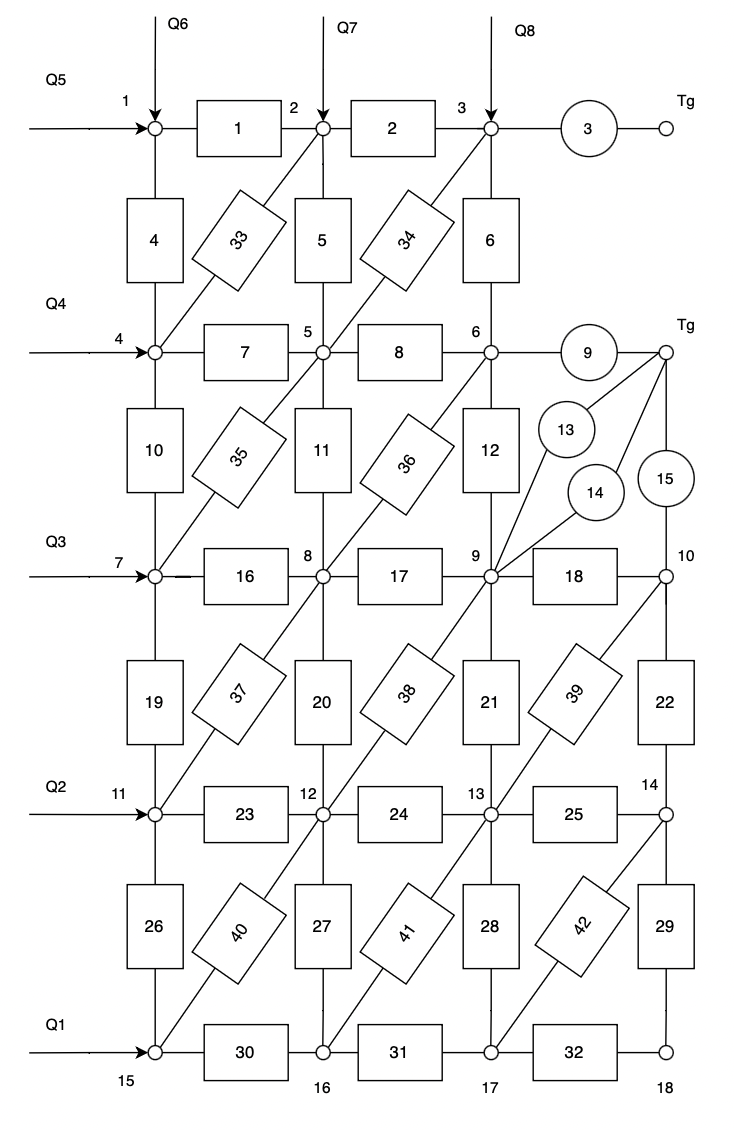
\includegraphics[scale=0.3]{pic1.png}
\end{center}

Сформируем глобальную матрицу $K$, где в качестве узлов $i,j,k$ будут тройки 

$[0,1,3], [1,2,4], [1,3,4], \dots$ 

В силу выбора размера тела, $l = 1,
l_{ij} = l_{ik} = l_{jk} = 1$ для любого узла. 

Код для решения задачи:
\begin{lstlisting}[language=Python]
import numpy as np
l = 1
S = 1/2
alpha = 10
q = 150
Tg = 25
lamb = 75
n = 18
K = np.zeros((n, n))
F = np.zeros(n)
nodes = np.array( [
            [0,1,3], [1,2,4], [1,3,4], [2,4,5], [3,4,6], 
            [4,5,7], [4,6,7], [5,7,8], [6,7,10], [7,8,11], 
            [8,9,12], [7,10,11], [8,11,12], [9,12,13], [10,11,14], 
            [11,12,15], [12,13,16], [11,14,15], [12,15,16], [12,16,17]])
            \end{lstlisting}
            \newpage
            \begin{lstlisting}[language=Python]
coordinates = np.array([ [4,0], [4,1], [4,2], [3,0], [3,1], 
	    [3,2], [2,0], [2,1], [2,2], [2,3], [1,0], [1,1], [1,2],
	    [1,3], [0,0], [0,1], [0,2], [0,3]])
bound_nodes_Q = np.array([[0,1], [1,2], [0,3], [3,6], [6,10], [10,14]])
bound_nodes_Tg = np.array([[2,5], [5,8], [8,9]])
for i, j, k in nodes:
    xi, yi = coordinates[i]
    xj, yj = coordinates[j]
    xk, yk = coordinates[k]
    ai = xj * yk - xk * yj
    aj = xk * yi - xi * yk
    ak = xi * yj - xj * yi
    bi = yj - yk
    bj = yk - yi
    bk = yi - yj
    ci = xk - xj
    cj = xi - xk
    ck = xj - xi
    k_x = l * lamb / (4 * S)
    K[i, i] += k_x * (bi ** 2 + ci ** 2)
    K[j, j] += k_x * (bj ** 2 + cj ** 2)
    K[k, k] += k_x * (bk ** 2 + ck ** 2)
    K[i, j] += k_x * (bi * bj + ci * cj)
    K[j, i] += k_x * (bi * bj + ci * cj)
    K[i, k] += k_x * (bi * bk + ci * ck)
    K[k, i] += k_x * (bi * bk + ci * ck)
    K[j, k] += k_x * (bj * bk + cj * ck)
    K[k, j] += k_x * (bj * bk + cj * ck)
for i, j in bound_nodes_Tg: 
    coef = alpha * l / 6
    K[i, i] += coef * 2
    K[j, j] += coef * 2
    K[i, j] += coef
    K[j, i] += coef
for i, j in bound_nodes_Tg: 
    F[i] += alpha * Tg * l / 2
    F[j] += alpha * Tg * l / 2
for i, j in bound_nodes_Q: 
    F[i] += l * q / 2
    F[j] += l * q / 2
L = np.linalg.cholesky(K)
y = np.linalg.solve(L, F)
T = np.linalg.solve(L.T, y)
\end{lstlisting}

\newpage
Решая СЛАУ, получим следующее распределение температур в узлах системы элементов:

\begin{table}[h]
    \centering
    \begin{tabular}{|c|c|c|c|c|c|c|c|c|c|}
        \toprule
        $T_1$&$T_2$&$T_3$&$T_4$&$T_5$&$T_6$&$T_7$&$T_8$&$T_9$&$T_{10}$\\ 
        \midrule
        62.54& 60.05& 56.52& 61.02 & 58.57& 55.13& 60.41& 58.09& 54.95& 53.28 \\ 
  \bottomrule	
    \end{tabular}
\end{table}
\begin{table}[h]
    \centering
    \begin{tabular}{|c|c|c|c|c|c|c|c|}
        \toprule
        $T_{11}$&$T_{12}$&$T_{13}$&$T_{14}$&$T_{15}$&$T_{16}$&$T_{17}$&$T_{18}$\\ 
        \midrule
        60.44& 58.41& 56.53& 55.44& 60.52& 58.60& 57.05& 57.05 \\ 
  \bottomrule
    \end{tabular}
\end{table}

\begin{center}
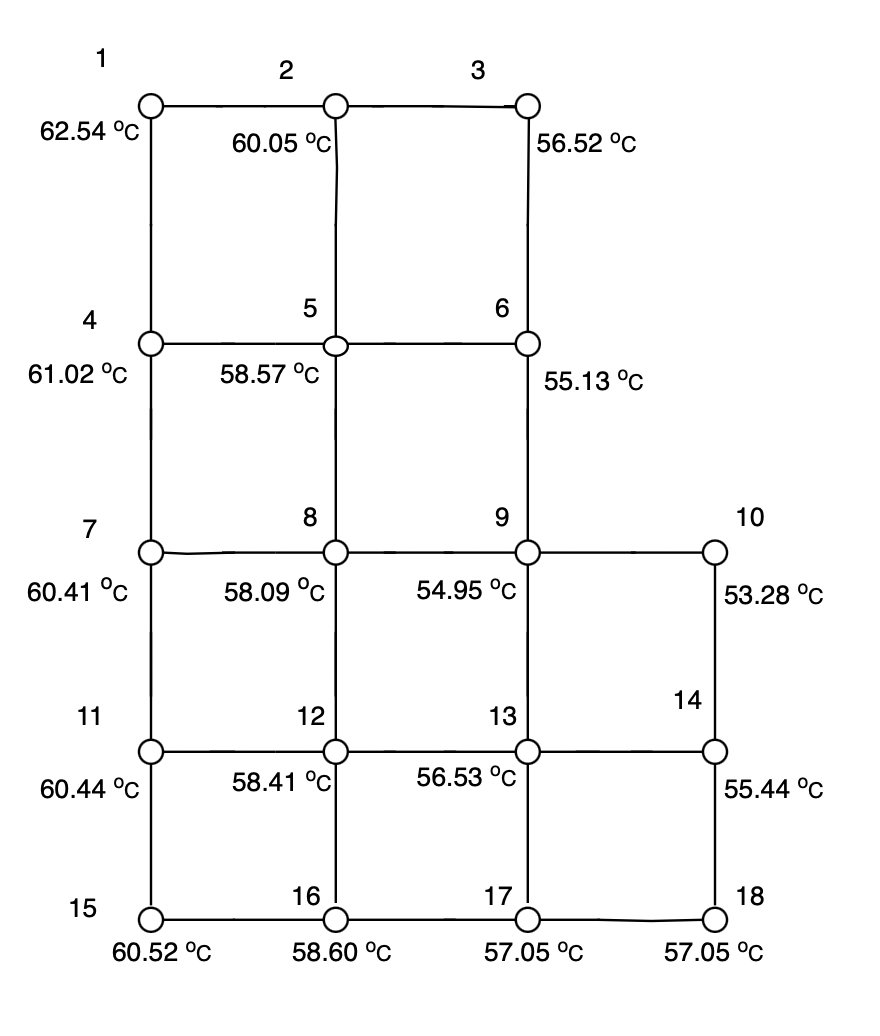
\includegraphics[scale=0.3]{T.png}
\end{center}

\end{enumerate}


\end{document}